Our metadata storage backend implements a modified version of \tfs
to pack together and manage all the metadata and small files,
hiding them from the underlying cluster file system.

\tfs \cite{TableFS} is a stacked file system which uses another file system
as an object store, and organizes all metadata and small files into a single
on-disk table using a Log-Structured Merge (LSM) tree \cite{ONeil1996, LevelDB}.
The reason for using LSM tree is that it buffers new and changed entries in
memory and translate small random disk writes into large sequential writes.
Because LSM tree can dramatically reduce random disk seeks,
it is a natural fit for metadata intensive workloads.
We decribe the structure of an LSM tree
and how LSM trees are used in \tfs in greater detail
in the following sections.

%\begin{figure}[!ht]
\begin{figure}[t]
\center
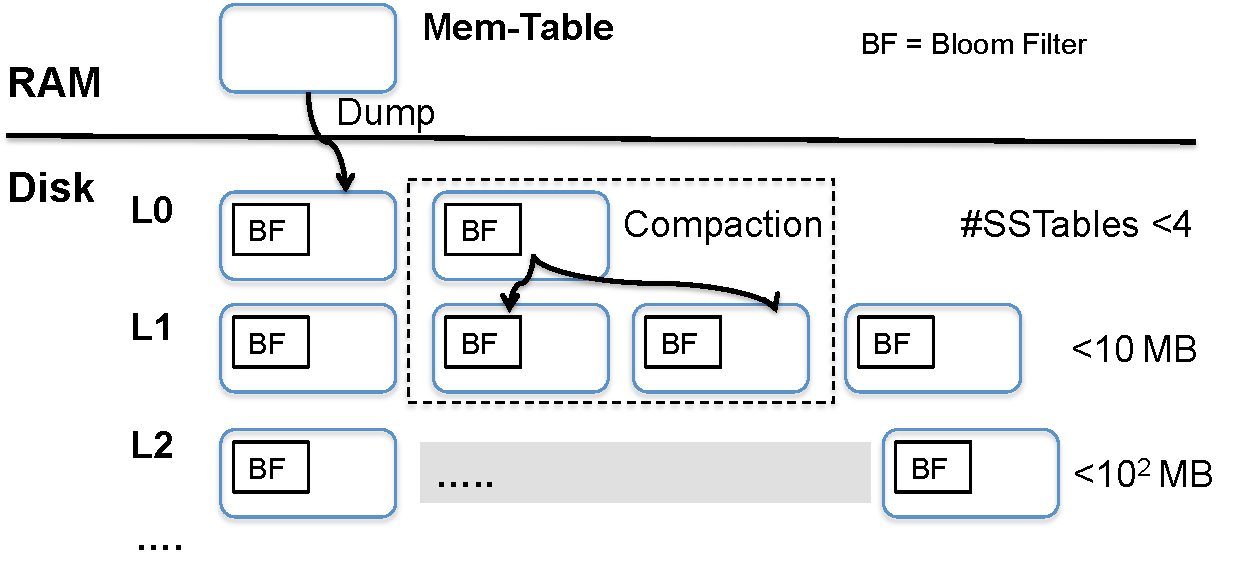
\includegraphics[scale=0.4]{figs/leveldb}
\vspace{10pt}
\caption{\textit{
LevelDB is an on-disk LSM-tree implementation that represents data in multiple 
files (called SSTables) containing sorted key-value pairs.
SSTables are grouped into different levels with lower-numbered levels
containing more recently inserted key-value pairs.
Finding a specific pair on disk may search up to all SSTables in level-0
and at most one in each higher-numbered level.
Compaction is the process of combining SSTables
by merge sort and moving combined SSTables into higher-numbered levels.
}}
%\vspace{10pt}
\hrule
\label{fig:leveldb}
\end{figure}


\textbf{LSM trees and LevelDB --}
\tfs uses an open-source implementation of an LSM tree called LevelDB
\cite{LevelDB}. LevelDB provides a simple key-value store interface,
supporting point queries and range queries. In LevelDB, by default,
a set of changes are spilled to disk when the total size of modified
entries exceeds 4 MB.  When a spill is triggered, called a
minor compaction, the changed entries are sorted, indexed and written to disk
in a format called an SSTable \cite{BigTable}.  These entries may then be
discarded from the in memory buffer. Discarded entries
can be reloaded by searching each SSTable
on disk, possibly stopping when the first match occurs if the SSTables are
searched most recent to oldest.  The number of SSTables that need to be
searched is reduced by maintaining the minimum and maximum key value
and a Bloom filter\cite{bloomfilter} on each,
but, with time, the cost of finding a record not in memory still increases.
Major compaction, or simply ``compaction",
is the process of combining multiple overlapping range SSTables
into a number of disjoint range SSTables by merge sort.

As illustrated in Figure \ref{fig:leveldb},
LevelDB extends this simple approach to further
reduce read costs by dividing SSTables into levels.
In 0-th level, each SSTable may contain entries with any key value,
based on what was in memory at the time of its spill.
The higher-numbered levels of LevelDB's SSTables are
the results of compacting SSTables from their own or lower-numbered levels.
In levels excepth the 0-th level, LevelDB maintains the following invariant:
the key range spanning each SSTable is disjoint from
the key range of all other SSTables at that level.
So querying for an entry in the higher levels
only needs to read at most one SSTable in each level.
LevelDB also sizes each of the higher levels differentially:
all SSTables have the same maximum size and
the sum of the sizes of all SSTables at level $L$ will not exceed $10^L$ MB.
This ensures that the number of level grows
logarithmically with increasing numbers of entries.

